\documentclass[10pt]{beamer}
\mode<presentation>
\usepackage{beamerthemesplit}
\usepackage{graphicx}
\usepackage{booktabs}
\usepackage{amsmath}
\usepackage{textpos}
\usepackage{pgfplots}
\usepackage{tikz}
\usepackage{hyperref}
\usepackage{caption}

% import citation package
\usepackage{biblatex}
\addbibresource{presentation.bib}
\AtBeginBibliography{\small}

\usetikzlibrary{shapes.geometric, arrows}
\usetikzlibrary {datavisualization} 
\pgfplotsset{compat=1.18, width = 7cm}
\usetikzlibrary{patterns}
\usetheme{Ilmenau} % AnnArbor, Ilmenau, Darmstadt, Dresden, CambridgeUS, Frankfurt, Singapore
\newtheorem{dn}{Định nghĩa}[section]
\newtheorem{dl}{Định lý}[section]
\newtheorem{tc}{Tính chất}[section]
\newtheorem{hq}{Hệ quả}[section]
\newtheorem{bd}{Bổ đề}[section]
\newtheorem{md}{Mệnh đề}[section]
\newtheorem{vd}{Ví dụ}[section]
\newtheorem{nx}{Nhận xét}[section]
\newtheorem{cy}{Chú ý}[section]
\newcommand{\dom}{\text{{\rm dom}}}
\newcommand{\epi}{\text{{\rm epi}}}
\newcommand{\Min}{\text{{\rm Min}}}
\setbeamertemplate{theorems}[numbered]
\setbeamertemplate{definitions}[numbered]
\setbeamertemplate{footline}[frame number]
\usepackage{algorithm}
\usepackage{color}
\usepackage{algorithmic}
\usepackage{footmisc}
\usepackage{indentfirst} 
\usepackage{comment}
\AtBeginEnvironment{proof}{%
  \setbeamercolor{block title}{use=example text,fg=white,bg=example text.fg!75!black}
  \setbeamercolor{block body}{parent=normal text,use=block title example,bg=block title example.bg!10!bg}
}
\renewcommand{\thefootnote}{\arabic{footnote}}
\usefonttheme{professionalfonts}
\setbeamercolor{normal text}{bg=white,fg=black}
\renewcommand{\thefootnote}{\arabic{footnote}}
\beamertemplatetransparentcoveredhigh
\usetheme[progressbar=frametitle]{metropolis}
\usepackage{appendixnumberbeamer}

\usepackage[utf8]{vietnam}

\usepackage{booktabs}
\usepackage[scale=2]{ccicons}

\usepackage{pgfplots}
\usepgfplotslibrary{dateplot}

\usepackage{xspace}
\newcommand{\themename}{\textbf{\textsc{metropolis}}\xspace}
\definecolor{mSybilaRed}{HTML}{990000}

\setbeamercolor{title separator}{
  fg=mSybilaRed
}

\setbeamercolor{progress bar}{%
  fg=mSybilaRed,
  bg=mSybilaRed!90!black!30
}

\setbeamercolor{progress bar in section page}{
  use=progress bar,
  parent=progress bar
}

\setbeamercolor{alerted text}{%
  fg=mSybilaRed
}

\setbeamertemplate{footline}
{
  \leavevmode
  \hbox{
  \begin{beamercolorbox}[wd=.15\paperwidth,ht=2.25ex,dp=1ex,center]{title in head/foot}
    \usebeamerfont{author in head/foot}\insertshortauthor
  \end{beamercolorbox}

  \begin{beamercolorbox}[wd=.7\paperwidth,ht=2.25ex,dp=1ex,center]{author in head/foot}
    \usebeamerfont{author in head/foot}\insertshorttitle
  \end{beamercolorbox}

  \begin{beamercolorbox}[wd=.15\paperwidth,ht=2.25ex,dp=1ex,center]{title in head/foot}
    \insertframenumber{} / \inserttotalframenumber
  \end{beamercolorbox}
  }
}


\title{Phương pháp giải bài toán Tối ưu tuyến tính nguyên}


\titlegraphic{\hfill 
\includegraphics[height=1cm]{logodhsg.png}}
%\titlegraphic{\hfill
\includegraphics[height=0.6cm]{sybila-logo/new.png}}
%\titlegraphic{\hfill
\includegraphics[height=0.6cm]{sybila-logo/old.png}}
%\titlegraphic{\hfill
\includegraphics[height=0.6cm]{sybila-logo/old-flat.png}}

\date{\today}
\author{Thực hiện: Đỗ Ngọc Minh Thư \& Nguyễn Chí Bằng}
\institute{Sinh viên lớp: DTU1221, Khóa: 22 @ Đại học Sài Gòn}

%\title{Metropolis}
\subtitle{Hướng dẫn: PGS.TS. Tạ Quang Sơn}
% \date{\today}
%\date{}
%\author{Matthias Vogelgesang}
%\institute{Center for modern beamer themes}
%\titlegraphic{\hfill
\includegraphics[height=1.5cm]{logo.pdf}}

\begin{document}
\begin{frame}
  \centering
  {\footnotesize
  ỦY BAN NHÂN DÂN THÀNH PHỐ HỒ CHÍ MINH\\
  TRƯỜNG ĐẠI HỌC SÀI GÒN}\\
  \phantom{space}\\
  {\normalsize BÁO CÁO ĐỀ CƯƠNG NGHIÊN CỨU KHOA HỌC\\
  NGÀNH: TOÁN ỨNG DỤNG}\\[-50pt]
  \titlepage
\end{frame}

\begin{frame}
    \frametitle{NỘI DUNG BÁO CÁO}
    \tableofcontents
\end{frame}

% Tai sao quan tam de tai?
% Lam duoc gi?
% Hoc duoc gi ?
% Du dinh tiep theo ?
% - - -
% Cơ sở lý thuyết và Mục tiêu
\section{Giới thiệu và Đặt vấn đề}

\begin{frame}{\bf Mục đích nghiên cứu}
\textbf{Tối ưu tuyến tính} là một nội dung quan trọng trong chương trình đào tạo Cử nhân Toán ứng dụng. Lý thuyết về việc giải bài toán tối ưu tuyến tính đã được cung cấp cho sinh viên. Tuy vậy, có nhiều bài toán tối ưu cần được giải với nghiệm nguyên. Chẳng hạn như:
\begin{itemize}
\item Bài toán tối ưu nhân lực.
\item Bài toán tối ưu vận chuyển hàng hóa.
\item Bài toán tối ưu áp dụng trong tin học.
\end{itemize}

\bigskip
Có một lý thuyết riêng cho việc xử lý các bài toán Tối ưu tuyến tính và \textcolor{red}{tìm nghiệm nguyên.}
\bigskip

{\it Mục đích của đề tài này là tìm hiểu một số phương pháp giải bài toán Tối ưu tuyến tính và tìm nghiệm nguyên cho bài toán.}
\end{frame}

\begin{frame}{\bf Tại sao cần có một lý thuyết riêng cho bài toán Tối ưu tuyến tính nguyên}

\begin{columns}
    \begin{column}{0.5\textwidth}
        \begin{equation*}
        \begin{array}{lll}            
        {\rm Max}&f(x)=2x_1+2x_2\\
        & \begin{cases}
        2x_1+x_2 \leq  8 \\
        x_1+3x_2 \leq 10 \\
        x_i\geq 0,\forall i=1,2.
        \end{cases} 
        \end{array}
        \end{equation*}
    \end{column}

    \begin{column}{0.5\textwidth}
        \begin{figure}
        \centering
        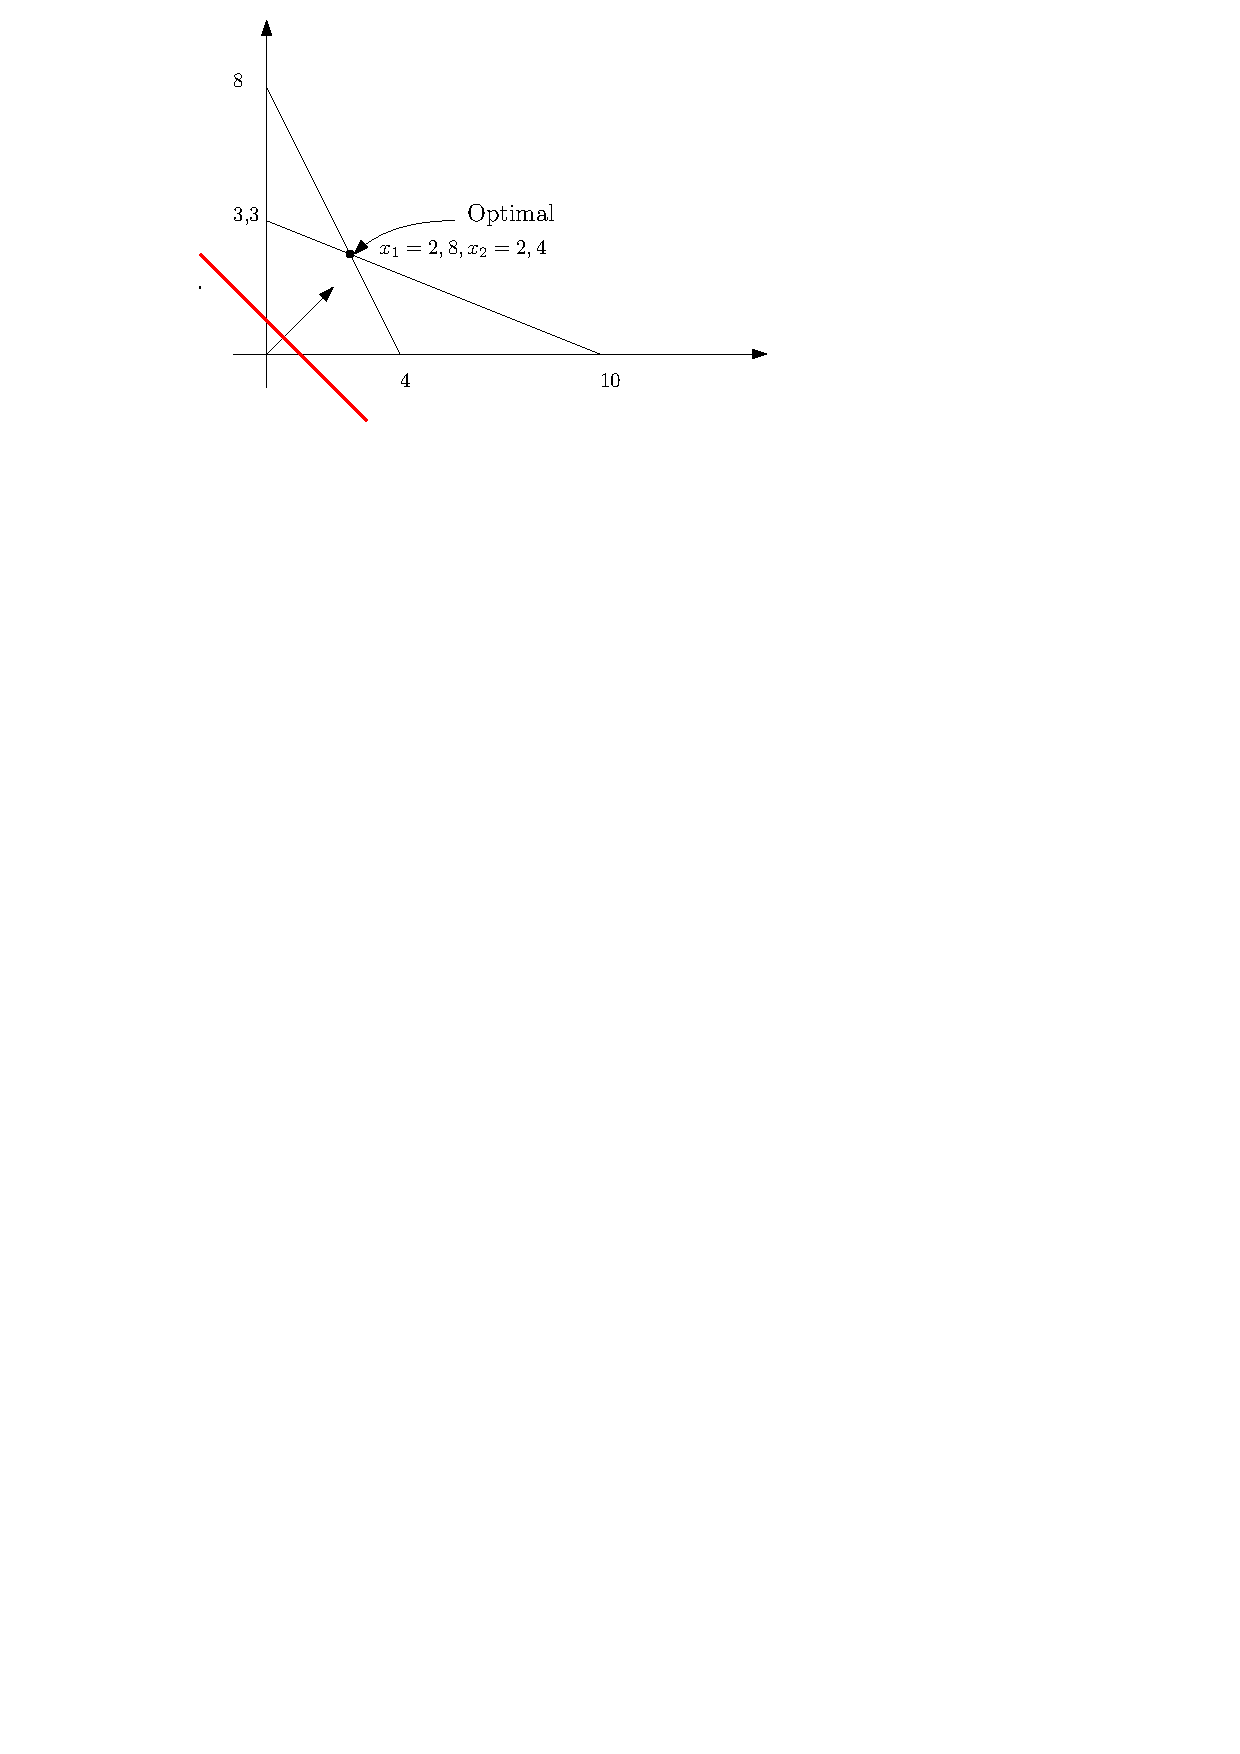
\includegraphics[width=1\linewidth]{Nhom1_hinh.pdf}
        \caption{Hình minh hoạ bài toán}
        \end{figure}
    \end{column}
\end{columns}
\end{frame}


\begin{frame}{\bf Nhận xét}
\begin{itemize}
\item<1-> Nếu giải bài toán trên bằng phương pháp thông thường, ta nhận được nghiệm $x_1=2.8$, $x_2=2.4$.
\medskip
      
      \item<2-> Nếu làm tròn nghiệm $x_1 \to 3$ và $x_2 \to 3$ thì điểm $(x_1,x_2)$ không còn thuộc miền chấp nhận được.
      
 \medskip
      
      \item<3-> Nếu làm tròn nghiệm $x_1 \to 2$ và $x_2 \to 2$ thì điểm $(x_1,x_2)$ chưa biết có phải nghiệm tối ưu hay không?
\end{itemize}
      
\bigskip
 \onslide<4->{\textcolor{red}{\bf Nếu giải bài toán QHTT rồi sau đó làm tròn số thì có thể  cho kết không như mong đợi.}}
   
\end{frame}







\begin{frame}{Tối ưu nguyên hoàn toàn (Pure integer linear program)}
    \begin{equation} \label{H}
        \begin{split}
        \onslide<1->{(H) \quad & z_h=c^Tx \quad \longrightarrow Max \\
                  & \left\{\begin{split}
                    &Ax \leq  b, \\
                    &x \geq 0, \text{ nguyên} \\
                    \end{split}\right.}    
        \end{split}
        \end{equation}            
    \begin{itemize} \small
    \item<2-> Trong đó $c^T=(c_1 \: c_2 \: \ldots \: c_n)$, $A$ là ma trận $m\times n$, $b=\begin{pmatrix}
        b_1 \\
        b_2 \\
        \vdots \\
        b_m
        \end{pmatrix}$, với $x\in Z^n$.
    \item<3-> Bài toán $(H)$ gọi là bài toán \textbf{Tối ưu nguyên hoàn toàn.}
    \item<4-> Tập $S_h:=\{x\in Z^n_+: Ax\leq b\}$ là tập nghiệm của bài toán Tối ưu nguyên hoàn toàn.
    \end{itemize}
\end{frame}

%model_1: hoan toan
\begin{frame} {Minh hoạ bài toán}
    \begin{equation}
        \begin{split}
        \quad & 2x_1 + 2x_2 \quad \longrightarrow Max \\
                    & \left\{\begin{split}
                    & x_1 + 3x_2 \leq 24 \\
                    & \frac{13}{3}x_1 + 2x_2 \leq 32.5 \\
                    &x_1 \geq 0, \text{ nguyên}. \\
                    &x_2 \geq 0, \text{ nguyên}. \\
                    \end{split}\right.    
        \end{split}
    \end{equation}            
\end{frame}
%cho bài toán ví dụ rõ số liệu
\begin{frame}
\begin{figure}[h]
    \centering
    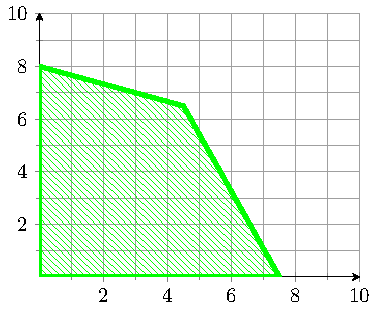
\includegraphics[width=0.7\linewidth]{nguyenhoantoan.pdf}
    \caption{Tập nghiệm của bài toán Tối ưu nguyên hoàn toàn}
\end{figure}
\end{frame}

\begin{frame}{Tối ưu nguyên bộ phận (Mixed integer linear program)}
\begin{equation}\label{2.4}
\begin{split}
\onslide<1->{(B) \quad & z_b=c^Tx+h^Ty \quad \longrightarrow Max \\
          & \left\{\begin{split}
            &Ax+Gy \leq  b, \\
            &x \geq 0, \text{ nguyên} \\
            &y \geq 0.
            \end{split}\right.}
\end{split}
\end{equation}    
\begin{itemize} \small
\item<2-> Trong đó $c^T=(c_1 \: c_2 \: \ldots \: c_n)$, $h^T=(h_1 \: h_2 \: \ldots \: h_p)$, $A$ là ma trận $m\times n$, $G$ là ma trận $m\times p$, $b=\begin{pmatrix}
    b_1 \\
    b_2 \\
    \vdots \\
    b_m
    \end{pmatrix}$, với $x\in Z^n$ và $y\in R^p$.
\item<3-> Bài toán $(B)$ gọi là bài toán \textbf{Tối ưu nguyên bộ phận.}
\item<4-> Tập $S_b:=\{(x,y)\in Z^n_+\times R^p_+: Ax+Gy\leq b\}$ là tập nghiệm của bài toán Tối ưu nguyên bộ phận.
\end{itemize}
\end{frame}
%cho bài toán ví dụ rõ số liệu
\begin{frame}{Minh hoạ bài toán}
   \begin{equation}
        \begin{split}
        \quad & x_1 + 2x_2 \quad \longrightarrow Max \\
                    & \left\{\begin{split}
                    & 5x_1 + \frac{15}{7}x_2 \leq 20 \\
                    & -2.4x_1 + \frac{30}{7}x_2 \leq 15 \\
                    &x_1 \geq 0, \text{ nguyên}. \\
                    &x_2 \geq 0. \\
                    \end{split}\right.    
        \end{split}
    \end{equation}            
\end{frame}

\begin{frame}
\begin{figure}[h]
    \centering
    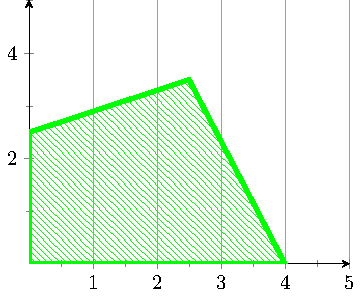
\includegraphics[width=0.7\linewidth]{nguyenbophan.pdf}
    \caption{Tập nghiệm của bài toán Tối ưu nguyên bộ phận}
\end{figure}
\end{frame}
    






































% DO NGOC MINH THU
\section{Phương pháp lát cắt Gomory}

\begin{frame}{Giới thiệu}
\vspace{-40pt}
Ta xét:\\
    \begin{equation}
     \begin{split}
         {(P)} & \quad {\rm Min}  \quad\langle c,x \rangle\\
          \rm{s.t} &\quad \left\{\begin{split}
            & Ax= b,\\
           & x_j \ge 0, j=1,2,...,n.\\
           \end{split}\right.
       \end{split}
   \end{equation}

  Ta ký hiệu tập $ F \subset \mathbb R^n$ là miền xác định của bài toán ${\rm (P)}.$
\end{frame}

\begin{frame}{Giới thiệu}
    \begin{equation}\label{BTNchinhtac}
     \begin{split}
         {(P^N)} & \quad {\rm Min}  \quad\langle c,x \rangle\\
          \rm{s.t} &\quad \left\{\begin{split}
            & Ax= b,\\
           & x_j \ge 0, j=1,2,...,n.\\
            & x_j \hspace{0.1cm} \text{nguyên}, j=1,2..,n_1\hspace{0.1cm}(n_1\le n).\\
           \end{split}\right.
       \end{split}
   \end{equation}
   
   Ta gọi:
   
   $P^N$ là bài toán tối ưu nguyên.
   
$F^N$ là miền xác định của bài toán.
\end{frame}

\section*{Ý tưởng về phương pháp cắt}
\begin{frame}{Sử dụng bao lồi của đa diện lồi}
Ta kí hiệu  $co(F)$ là bao lồi của đa diện lồi $F$
    \begin{dl}
   Giả sử $F$ là một đa diện lồi,\hspace{0.1cm} $F^N$ là tập các điểm nguyên của nó, 
$R \hspace{0.1cm} \text{là bao lồi của} F^N$( tức là $R= co(F^N)$) khi đó:\\
    1) $R$ là một đa diện nguyên.\\
    2) $R^N=F^N$.\\
    3) Tập $R^\ast$ các phương án chấp nhận được của đa diện $R$ chứa trong $R^N$:
    $$R^{\ast} \subseteq R^N.$$
\end{dl}
\end{frame}

\begin{frame}{Sử dụng bao lồi của đa diện lồi}
    \begin{hq}
     Giả sử $X$  là phương án tựa tối ưu của bài toán $Q$ (bài toán tối ưu tuyến tính có miền xác định là đa diện $R$, khi đó $X$ cũng là phương án tối ưu của bài toán  $P^N$. Vì vậy để giải bài toán quy hoạch tuyến tính nguyên $P^N$ ta đi giải bài toán $Q$.\\
\end{hq}
\begin{dl}
 Giả sử $L$ là một đa diện lồi, $U$ là một đa diện lồi nguyên và $U^N= F^N$, khi đó :
 $$U = R = co(F^N).$$
    \end{dl}
\end{frame}

\begin{frame}{Sử dụng bao lồi của đa diện lồi}
    Ví dụ minh họa:\\
    \begin{tabular}{|c|c|c|}
    \hline
     BÀI TOÁN $(P^N)$  & BÀI TOÁN $(P)$& BÀI TOÁN $(Q)$  \\
     \hline
       $Max (x_1+x_2)$  & $Max (x_1+x_2) $ &$Max (x_1+x_2)$ \\
$2x_1+11x_2\le 38$ \quad (a) & $2x_1+11x_2 \le 38$  \quad (a) & $x_2\le 3$\\
$x_1+x_2\le 7$\quad (b) &$x_1+x_2\le 7$\quad (b) & $x_1+x_2\le 5$\\
$4x_1-5x_2\le 5$ \quad c & $4x_1-5x_2\le 5$\quad (c) & $x_1-x_2\le 1$\\
$x_j\ge 0$ & $x_j\ge 0$ & $x_j\ge 0$\\
$x_j$ nguyên & &\\
\hline 
$Max= 5$& $Max=7$ &$Max=5$\\
Tối ưu là 2 điểm & Tối ưu là một đoạn & Tối ưu là đoạn\\
$(2;3);(3;2)$&$[(\frac{13}{3},\frac{8}{3}); (\frac{40}{9};\frac{23}{9})]$&$[(2;3);(3;2)]$\\
\hline
    \end{tabular}
\end{frame}

\begin{frame}{Sử dụng bao lồi của đa diện lồi}
    \begin{figure}[h]
        \centering
        \includegraphics[width=0.65\linewidth]{ảnh 1.pdf}
        \caption{Ảnh minh họa }
        \label{fig:enter-label}
    \end{figure}
\end{frame}

\begin{frame}{Khái niệm lát cắt đúng}
     Giả sử bài toán $P^N$là bài toán quy hoạch nguyên nào đó và phương án tựa tối ưu của bài toán quy hoạch tuyến tính tương ứng $X$ không thoả mãn điều kiện 
nguyên, tức là $X \notin  F^N$.\\
Khi đó, bất đẳng thức:
    $$\sum _j a_jx_j \le \beta$$\label{latcat}
    được gọi là lát cắt đúng nếu thỏa mãn hai điều kiện.\\
    
       \textbf{ 1) Điều kiện cắt:} \\
        $X$ không thỏa mãn điều kiện \eqref{latcat}, tức là $Ax > \beta$.\\
    \textbf{2) Điều kiện đúng:}\\
       Nếu $X$ là phương án của bài toán tối ưu nguyên thì $X$ thỏa mãn điều kiện \eqref{latcat}, tức là 
 $F^N \subset \{X\mid aX\le \beta\}$.\\
    \end{frame}

    \begin{frame}{Khái niệm lát cắt đúng}
         Nói cách khác, lát cắt thêm vào sẽ không cắt đi một phương án nguyên nào của bài toán.\\
    \vspace{0.5cm}
    \begin{figure}[h]
        \centering
        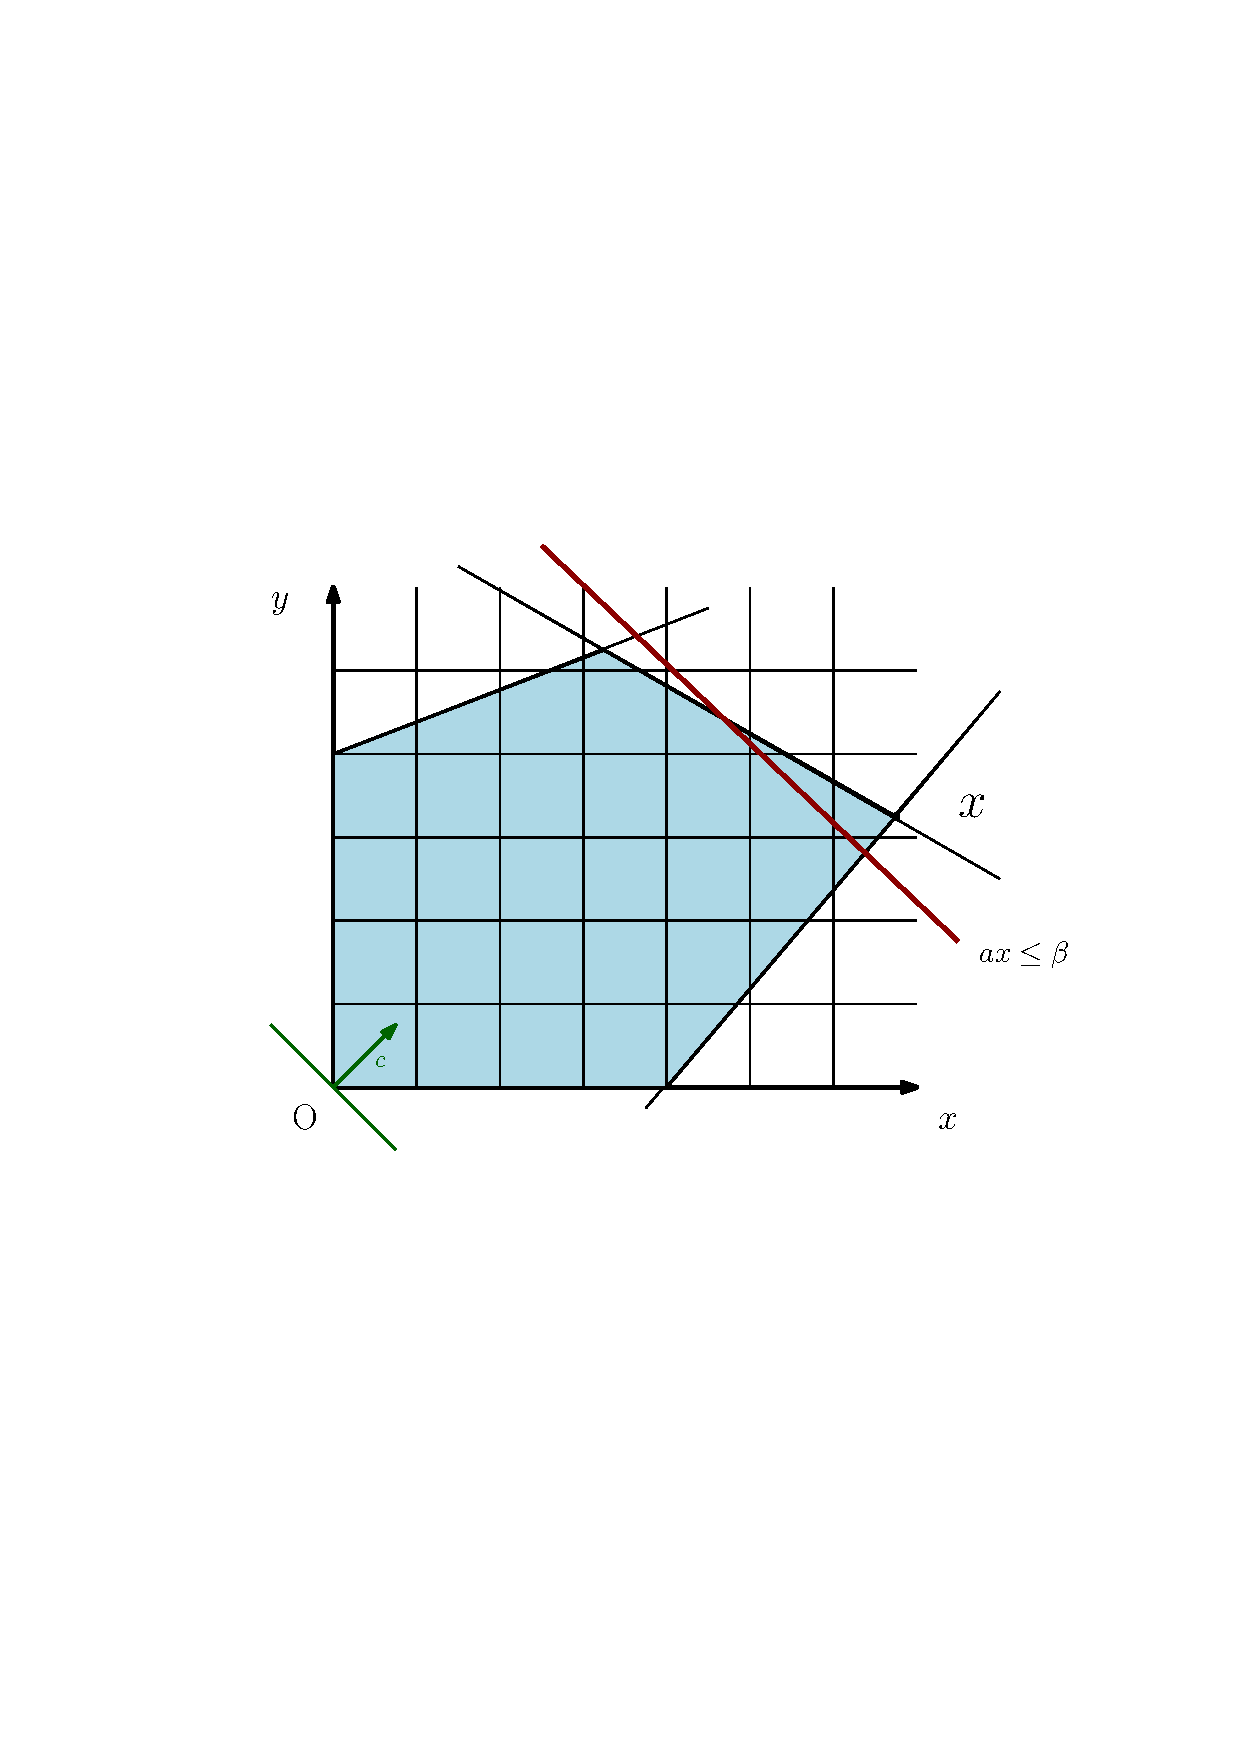
\includegraphics[width=0.5\linewidth]{anh2.pdf}
       
    \end{figure}
    \end{frame}

    \begin{frame}{ Ý tưởng phương pháp cắt của Danzig}
         Việc giải một bài toán $P^N$ là một quá trình gồm nhiều bước:\\
a) Ở bước thứ $r$,  giải bài toán bài toán quy hoạch tuyến tính phụ 
 $P_r, r = 0,1,... 
… \text{với}   F_0=F $\\
b) Tập các điểm  nguyên của tất cả các đa diện lồi là như nhau:
$$F_0^N=F_1^N=F_2^N=...=F_r^N=.......$$\\
Do đó, nếu phương án tối ưu $X^*_r$ của bài toán $P_r$ thoả mãn điều kiện nguyên thì nó cũng là phương án tối ưu $X_0$ của bài toán xuất phát $P^N_0$ và quá trình kết thúc.\\
\end{frame}

    \begin{frame}{ Ý tưởng phương pháp cắt của Danzig}
c)  Nếu $X^*_r$ không thoả mãn điều kiện nguyên thì $X^*_r$ không phải là 
phương án của bài toán $P_{r+1}$, tức là $X_r^*\notin F_{r+1}$.\\Chuyển từ bước $r$ sang bước $r+1$, tức là chuyển từ bài toán $P_r$ sang 
 $P_{r+1}$ khi $X^*_r$ không nguyên được thực hiện nhờ một lát cắt đúng $a_rx \le \beta_r$.\\
Việc bổ sung lát cắt này vào ràng buộc của bài toán $P_r$ sẽ chuyển đa diện lồi $F_r$ thành $F_{r+1}$.\\
    \end{frame}
\section*{Thuật toán Gomory}
    \begin{frame}{Cơ sở lý thuyết}
        Ta xét bài toán tối ưu nguyên hoàn toàn:\\
\begin{equation}\label{Gomory1}
     \begin{split}
      (P^N) \quad    & {\rm{Max}} \langle c,x \rangle\\
          \rm{s.t} &\left\{\begin{split}
            & Ax= b,\\
           & x_j \ge 0, j=1,2,...,n.\\
            & x_j \text{nguyên}, j=1,2..,n.\\
           \end{split}\right.
       \end{split}
   \end{equation}
   \begin{dn}
     Giả  sử hệ véc-tơ $\{A^j,j\in J\}$ là cơ sở tương ứng với phương án cực biên ban đầu của bài toán $P^N$, các véc-tơ $A^j$ và các biến $x_j$ với $j\in J$ được gọi là các véc tơ cơ sở và biến cơ sở; còn các véc-tơ $A^j$ và các biến $x_j$ mà $j \notin J$ được gọi là các véc-tơ tự do và các biến tự do (biến phi cơ sở).\\  
   \end{dn}
    \end{frame}

    \begin{frame}{Cơ sở lý thuyết}
         Giả sử $X$ là phương án  tối ưu của bài toán $P^N$, từ đó ta có thể biểu diễn các biến cơ sở qua Các biến phi cơ sở:\\
   \begin{equation}\label{2.4}
       x_{i}=x_{i0} + \sum_{j \in N} x_{ij}(-x_j), i=\overline{0,m}.
   \end{equation}
    \end{frame}

    \begin{frame}{Cơ sở lý thuyết}
        \begin{dl}
        Giả sử $X$ có $x_{i0}$ không nguyên với $1\le i\le n$ và:\\
        1)\begin{equation}\label{2.5}
            z_i\equiv z_i(X)= -\{x_{i0}\} + \sum_{j \in \mathbb {N} }(-\{x_{ij}\})(-x_{j}), i=\overline{1,n}.
        \end{equation} \\
        2) $x$ là phương án của bài toán $P^N$.\\
        Khi đó:\\
        a) $z_i \hspace{0.1cm} \text{nguyên}$.\\
        b) $z_i \ge 0$. 
        \end{dl}
    \end{frame}

    \begin{frame}{Cơ sở lý thuyết}
        \begin{hq}
        Giả sử $X(L,C)$ không thoả mãn điều kiện nguyên, như vậy đối 
với $i$ nào đó $(1\le i \le 0) \hspace{0.1cm} x_{i0}$ không nguyên . Khi đó các hệ thức \eqref{2.5}  và $z_i \ge 0$ xác định một lát cắt đúng.
    \end{hq} 
    \end{frame}

\begin{frame}{Dấu hiệu bài toán không có lời giải}
\begin{figure}[h]
    \centering
    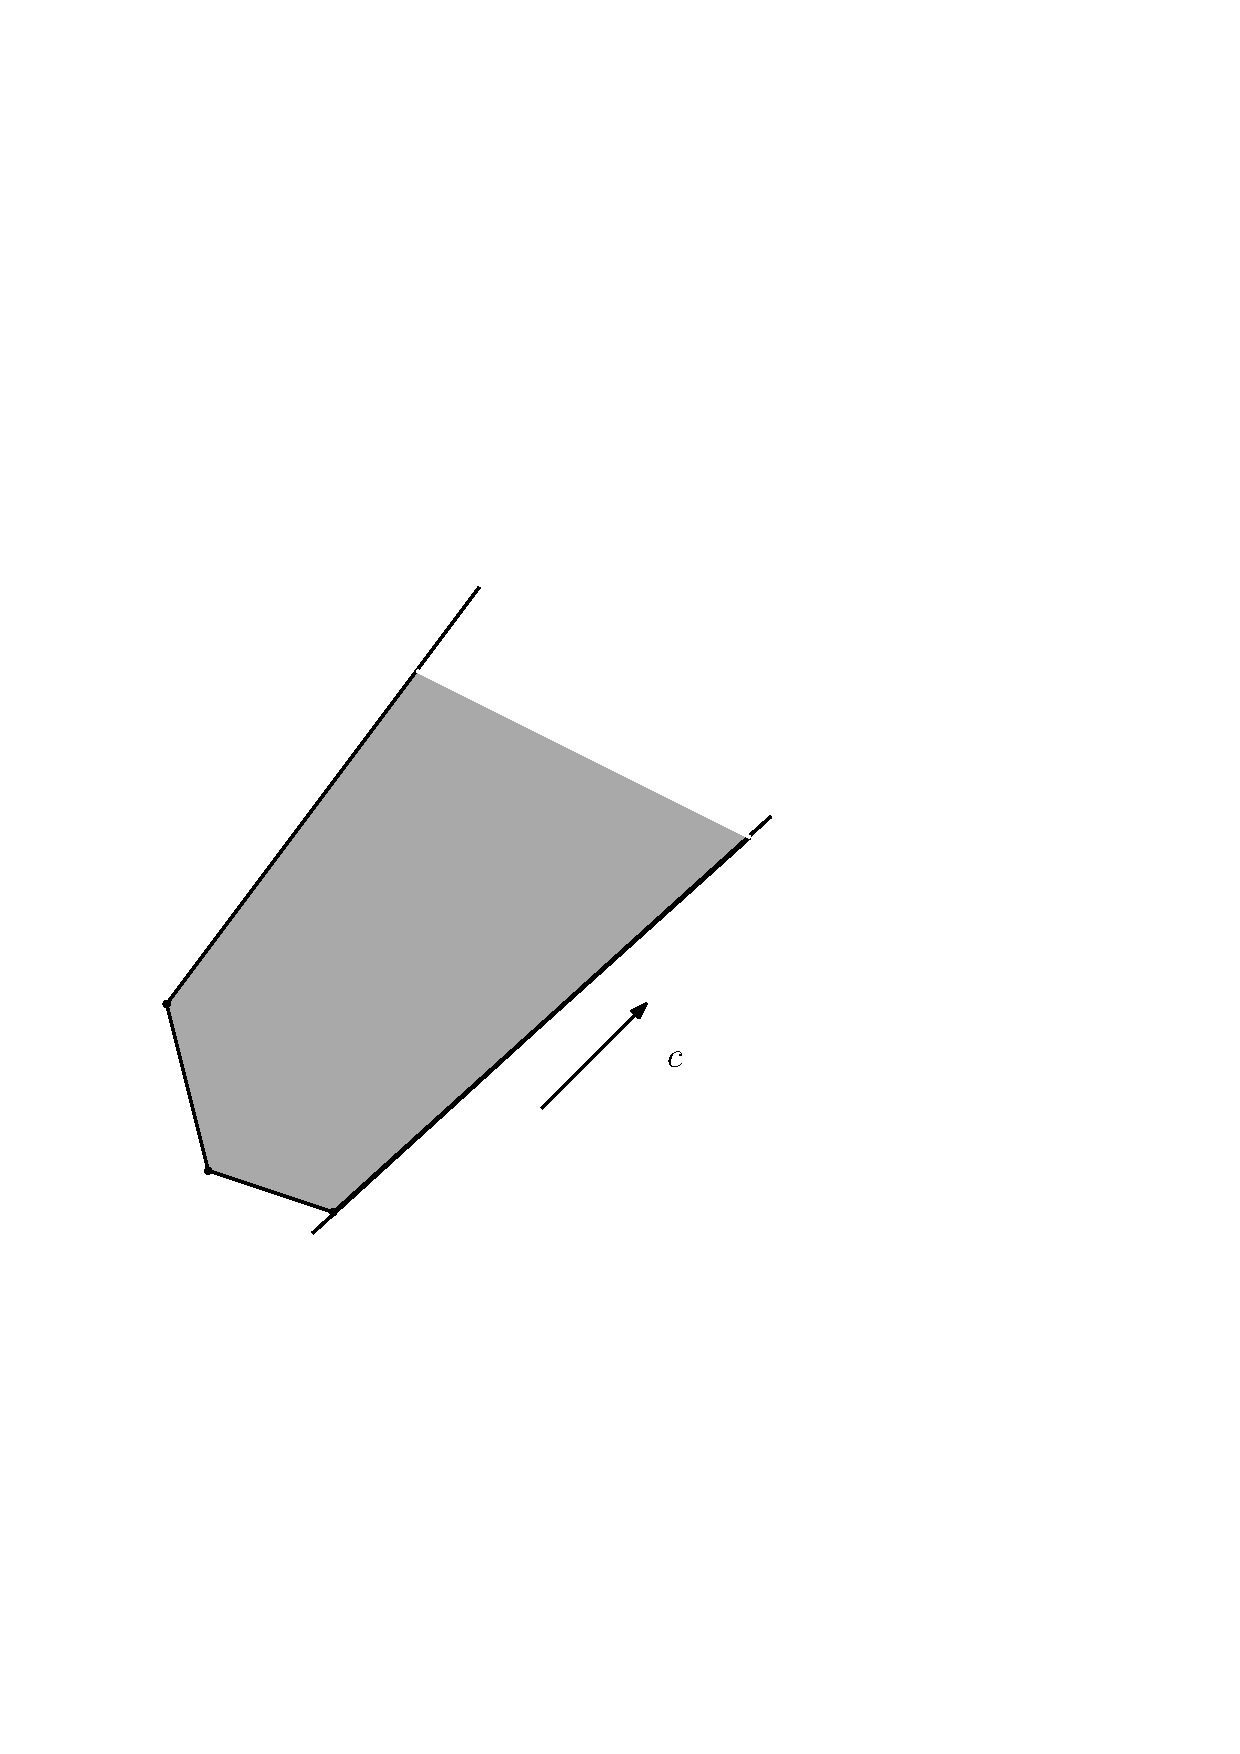
\includegraphics[width=0.45\linewidth]{anh3.pdf}
    \caption{$\overline{P}$ không có lời giải}
\end{figure}
    \end{frame}

    \begin{frame}{Dấu hiệu bài toán không có lời giải}
        Về sau ta sẽ giả thiết:\\
1) Hàm mục tiêu $x_0\equiv CX$ bị chặn trên $F$.\\
2) Nếu tập hợp các phương án tối ưu của $P$ khác trống thì nó phải bị chặn, tức là nếu bài toán $P$ giải được thì bài toán $\overline{P}$ cũng giải 
được.\\
    \end{frame}

    \begin{frame}{Thuật toán Gomory}
        \textbf{Bước 1:}
Giải bài toán $P\equiv P_0$ đã cho bằng phương pháp đơn hình đối ngẫu.\\
- Nếu $P_0$ không giải được thì $P_0^N$ cũng không giải được.\\
- Nếu  $P_0$ giải được và nghiệm của nó thỏa mãn điều kiện nguyên thì nó cũng là phương án tối ưu của $P^N_0$, còn nếu chưa thỏa điều kiện thì chuyển sang bước 2.\\
       
    \end{frame}

    \begin{frame}{Thuật toán Gomory}
     \textbf{Bước 2:}
Chọn dòng đầu tiên ứng với thành phần không nguyên:\\
$k=min\{i|i\in \{1,...,n\},x_{i0}^r \text{không nguyên}\}$ và xây dựng lát cắt đúng:\\
$$   \begin{cases}\label{latcat}
    x_{n+r+1}= -\{x_{k0}^r\} + \sum_{j\in N_r}(-\{x_{kj}^r\} )(-x_j)\\
    x_{n+r+1} \ge 0\\
    x_{n+r+1} \hspace{0.1cm} \text{nguyên}
\end{cases}$$
Thêm lát cắt vào bảng đơn hình và tiếp tục giải bài toán $P^N_{r+1}$.\\
        \textbf{Bước 3:}
Sau khi tính toán với lát cắt nếu được phương án tối ưu thỏa mãn điều kiện nguyên thì thuật toán dừng lại. Nếu không thỏa mãn thì quay lại bước 2 cứ lần lượt như vậy thực hiện các bước lặp $r \ge 0$ cho đến khi thỏa mãn điều kiện.\\

    \end{frame}

     \begin{frame}{Tính hữu hạn của thuật toán}
         \begin{dl}
Giả sử có các điều kiện sau:\\
1) Tính nguyên của hàm mục tiêu $x_0\equiv CX$ được đảm bảo và $x_0$ được xét khi chọn dòng xây dựng lát cắt đúng.\\
2) Một trong các khẳng định sau là đúng:\\
i) Hàm mục tiêu $x_0$ bị chặn dưới trên $F_0$.\\ 
ii) Bài toán $P^N_0$ có ít nhất một phương án $X'$.\\
 Khi đó thuật toán Gomory thứ nhất kết thúc sau một số hữu hạn bước lặp lớn.
 \end{dl}
\end{frame}









\section{Phương pháp Land-Doig}

\begin{frame}{Ý tưởng phương pháp Land-Doig}
    \begin{itemize}
    \item \textbf{Phương pháp Land-Doig (Nhánh cận)}: Chia bài toán gốc thành các bài toán nhỏ và xử lý đến khi tìm ra kết quả tối ưu.
    \medskip
    \item \textbf{Cách hoạt động}: Thuật toán Land-Doig là một khung thuật toán chia bài toán thành \textcolor{red}{\textbf{các bài toán con}} và duyệt qua từng bài toán. Từ giải pháp ban đầu, thuật toán mở rộng các nhánh (tập hợp con các bài toán) và duyệt có hệ thống như một mê cung.
    \medskip
    \item \textbf{Ý tưởng cốt lõi}:
    \begin{itemize} 
        \item \textcolor{red}{\textbf{Phân nhánh}}: Mỗi nhánh đại diện cho một tập con các bài toán.
        \item \textcolor{red}{\textbf{Gọt}}: Loại bỏ nhánh không thỏa điều kiện nghiệm, giúp tìm giải pháp tối ưu hiệu quả.
    \end{itemize}
    \end{itemize}
\end{frame}

\begin{frame}{Bài toán quan tâm}
\begin{equation}\label{P}
\begin{split}
\onslide<1->{(P) \quad & z_p=c^Tx+h^Ty \quad \longrightarrow Max \\
            & \left\{\begin{split}
                &Ax+Gy \leq  b, \\
                &x,y \geq 0.
            \end{split}\right.}    
\end{split}
\end{equation}
\begin{itemize}
\item<2-> Trong đó $(P)$ là bài toán $(B)$ (hoặc $(H)$) với nghiệm thuộc tập số thực.
\item<3-> Bài toán $(P)$ là một bài toán \textbf{Tối ưu tuyến tính thông thường} hay gọi đơn giản là bài toán Tối ưu tuyến tính (Natural linear programming relaxation).
\item<4-> Tập $S_p:=\{(x,y)\in R^n_+\times R^p_+: Ax+Gy\leq b\}$ là tập nghiệm của bài toán Tối ưu tuyến tính.
\end{itemize}
\end{frame}

\begin{frame}{Mục tiêu} %aka Lí do chọn bài toán
\onslide<1->{Giả sử ta nhận được tập phương án tối ưu của bài toán $(B)$ sau hữu hạn lần giải, ký hiệu $(x_b, y_b)$ và giá trị tối ưu là $z_b$ thì ta có nhận xét sau:}
\onslide<2->{\begin{nx} \label{nx}
\begin{itemize}
\item Nếu $S_b \subseteq S_p$ thì ta luôn nhận được $z_b \leq z_p$ và phương án có thể cải thiện.
\item Nếu $S_b = S_p$ thì ta nhận được $z_b = z_p$ và bài toán được giải.
\end{itemize}    
\end{nx}}
\bigskip
\onslide<3->{Vì thế, ta chọn xử lý bài toán $(B)$ (hoặc $(H)$) thông qua bài toán $(P)$ bằng cách cải thiện phương án thu được từ bài toán $(P)$ sao cho thoả điều kiện của bài toán $(B)$ (hoặc $(H)$).}
\end{frame}

\begin{frame}{Ví dụ}
        \small
        \begin{equation} \label{baitoannguyenloi}
        \begin{split}
            (H) \quad & 5.5x_1 + 2.1x_2 \quad \longrightarrow Max \\
            & \left\{\begin{array} {cccc}
            -1x_1 &+ x_2 &\leq& 2 \\
            8x_1 &+ 2x_2 &\leq& 17 \\
            x_1 &&\geq & 0, \text{ nguyên} \\
            &x_2 &\geq& 0, \text{ nguyên}. \\
            \end{array}\right.
            \Longrightarrow
            \left\{\begin{array} {ccc}
            \color{red}x_1 & \color{red}=& \color{red} 1.3 \\
            \color{red} x_2 &\color{red}=& \color{red}3.3 \\
            z &=&14.08
        \end{array}\right.
        \end{split}
        \end{equation}
    \vspace{0.5cm}
    \center
    \Large
    Phương án có thể cải thiện.
\end{frame}


\begin{frame}{Ví dụ}
    \begin{equation} \label{baitoannguyenhet}
    \begin{split}
        (H) \quad & 3x_1 + 4x_2 \quad \longrightarrow Max \\
        & \left\{\begin{array} {cccc}
        2.5x_1 &+ \frac{15}{4}x_2 &\leq& 20 \\
        x_1 &+ \frac{5}{3}x_2 &\leq& \frac{50}{3} \\
        x_1 &&\geq &0, \\
        &x_2 &\geq& 0. \\
        \end{array}\right.
        \Longrightarrow
        \left\{\begin{array}{ccc}
        \color{blue} x_1 &\color{blue} = &\color{blue} 5 \\
        \color{blue} x_2 &\color{blue} = & \color{blue} 7 \\
        z& =&43
    \end{array}\right.
    \end{split}
    \end{equation}
    \vspace{0.5cm}
    \center
    \Large
    Bài toán được giải.
\end{frame}

\section*{Thuật toán Land-Doig}

\begin{frame}{Phương pháp xác định cận}
Ta gọi $x_j$ với $1 \leq j \leq n$ là nghiệm thu được từ bài toán $(P)$.
\begin{dl}\label{cmnguyen}
\begin{itemize}
\item Với mỗi $x_j \in \mathbb{R}$, tồn tại duy nhất số nguyên $k \in \mathbb{Z}$ sao cho $k \leq x_j < k+1$.
\begin{itemize}
\item Giá trị $k$ khi đó ta gọi là phần nguyên nhỏ nhất của $x_j$, ký hiệu là $\lfloor x_j \rfloor$.
\item Giá trị $k+1$ gọi là phần nguyên lớn nhất của $x_j$, ký hiệu là $\lceil x_j \rceil$.
\end{itemize}
\end{itemize}
\end{dl}
\bigskip
\begin{vd}
Ta có $x_1=3.3$, vậy khi đó phần nguyên nhỏ nhất của $x_1$ là $\lfloor x_1 \rfloor = 3$ và phần nguyên lớn nhất là $\lceil x_1 \rceil =4$.
\end{vd}
\end{frame}

\begin{frame}{Phương pháp xử lý bài toán}
\large
\begin{itemize}
\item<1-> Từ bài toán minh hoạ \eqref{baitoannguyenloi} và \eqref{baitoannguyenhet}, ta thấy rằng nếu $\exists x_j \notin \mathbb{Z}$, thì ta có thể tiếp tục cải thiện phương án cho đến khi $\forall x_j \in \mathbb{Z}$. 
\bigskip
\item<2-> Nếu nghiệm thu được là $x_j \notin \mathbb{Z}$ ta thiết lập được 2 bài toán con từ bài toán $(P)$ ban đầu, ký hiệu $(P_1)$ và $(P_2)$.
\end{itemize}
\end{frame}

\begin{frame}
\begin{equation}
    \begin{split}
    (P_1) \quad & z_1=c^Tx+h^Ty \quad \longrightarrow Max \\
                & \left\{\begin{split}
                    &Ax+Gy \leq  b \\
                    &\color{blue} x_j \leq \lfloor x_j \rfloor , \\
                    &x,y \geq 0.
                \end{split}\right.    
    \end{split}
\end{equation}
\begin{itemize}
\item Tập $S_1:=S_p \cap \{ (x,y): x_j \leq \lfloor x_j \rfloor \}$ là tập nghiệm tối ưu của bài toán con $(P_1)$.
\end{itemize}
\end{frame}

\begin{frame}
\begin{equation}
    \begin{split}
    (P_2) \quad & z_2=c^Tx+h^Ty \quad \longrightarrow Max \\
                & \left\{\begin{split}
                    &Ax+Gy \leq  b \\
                    &\color{blue} x_j \geq \lceil x_j \rceil , \\
                    &x,y \geq 0.
                \end{split}\right.    
    \end{split}
\end{equation}
\begin{itemize}
\item Tập $S_2:=S_p \cap \{ (x,y): x_j \geq \lceil x_j \rceil \}$ là tập nghiệm tối ưu của bài toán con $(P_2)$.
\end{itemize}
\end{frame}

\begin{frame}{Điều kiện nghiệm}
\begin{itemize}
\item<1-> Nếu tồn tại $(P_i)$ với $i=1,2$ không giải được $(S_i = \emptyset )$, ta gọi bài toán \textbf{vô nghiệm}.
\medskip
\item<2-> Giả sử $x^{(i)}$ là nghiệm tối ưu của bài toán $(P_i)$ và giá trị tối ưu là $z_i$ với $i = 1,2$.
\begin{itemize}
\item<3-> Nếu $\forall x^{(i)} \in Z^n_+$, ta nói $S_i$ là tập nghiệm thoả mãn bài toán tối ưu nguyên bộ phận, $z^*_i$ là giá trị tối ưu và bài toán con $(P_i)$ được giải \textbf{(gọt bởi nghiệm nguyên)}.
\item<4-> Nếu $\exists x^{(i)} \notin Z^n_+$ đồng thời $z_i \leq z^*_i$, ta dừng phân nhánh và bỏ qua bài toán \textbf{(gọt bởi cận)}.
\item<5-> Nếu $\exists x^{(i)} \notin Z^n_+$ đồng thời $z_i > z^*_i$, bài toán chưa tối ưu và có thể tiếp tục cải thiện.
\end{itemize}
\end{itemize}
\medskip
\onslide<6->{\begin{cy}
Ta gọi $x_j^{(i)}$ là biến thứ $j$ của bài toán thứ $i$.
\end{cy}}
\end{frame}

\begin{frame}{Ví dụ minh hoạ}
    \begin{equation*}
        \begin{split}
            (H) \quad &z_p= 5.5x_1 + 2.1x_2 \quad \longrightarrow Max \\
            & \left\{\begin{array}{cccc}
            -x_1 &+ x_2 &\leq& 2 \\
            8x_1 &+ 2x_2 &\leq& 17 \\
            x_1 &&\geq& 0, \text{ Nguyên}\\
            &x_2 &\geq& 0, \text{ Nguyên}. \\
            \end{array}\right. \\
        \end{split}
    \end{equation*}
\end{frame}

\begin{frame}
    Giải bài toán bằng phương pháp đơn hình thông thường ta được nghiệm $x_1 =1.3$, $x_2 = 3.3$ và $z_p=14.08$.
    \vspace{0.5cm}
\begin{figure}[h]
    \centering
    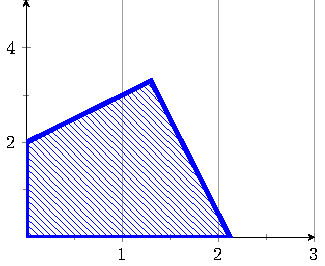
\includegraphics[width=0.4\linewidth]{hinh1.pdf}
    \caption{Tập nghiệm của bài toán}
\end{figure}
\end{frame}

%template to copy-paste
\begin{frame}
\onslide<1->{Chọn $x_1=1.3$ để cải thiện phương án, ta thu được 2 bài toán con sau:}
\bigskip
\begin{columns}
\begin{column}{0.5\textwidth}<2->
    \small
    \begin{equation*}
        \begin{split}
            (P_1) \quad &z_1= 5.5x^{(1)}_1 + 2.1x^{(1)}_2 \\
            & \left\{\begin{array} {cccc}
            -x^{(1)}_1 &+ x^{(1)}_2 &\leq& 2 \\
            8x^{(1)}_1 &+ 2x^{(1)}_2 &\leq& 17 \\
            \color{blue} x^{(1)}_1 && \color{blue} \leq &\color{blue} 1 \\
            x^{(1)}_1 &&\geq& 0 \\
            &x^{(1)}_2 &\geq& 0. \\
            \end{array}\right. \\
        \end{split}
    \end{equation*}
\end{column}
\begin{column}{0.5\textwidth}<2->
   \small
   \begin{equation*}
        \begin{split}
            (P_2) \quad &z_2= \hspace{0.1cm} 5.5x^{(2)}_1 + 2.1x^{(2)}_2  \\
            & \left\{\begin{array} {cccc}
            -x^{(2)}_1 &+ x^{(2)}_2 &\leq &2 \\
            8x^{(2)}_1 &+ 2x^{(2)}_2 &\leq &17 \\
            \color{blue} x^{(2)}_1 &&\color{blue}\geq&\color{blue} 2 \\
            x^{(2)}_1 &&\geq& 0 \\
            &x^{(2)}_2 &\geq& 0. \\
            \end{array}\right. \\
        \end{split}
    \end{equation*}
\end{column}
\end{columns}
\end{frame}

\begin{frame}
    \begin{equation*}
        \begin{split}
            (P_1) \quad &z_1= 5.5x^{(1)}_1 + 2.1x^{(1)}_2 \\
            & \left\{\begin{array} {cccc}
            -x^{(1)}_1 &+ x^{(1)}_2 &\leq& 2 \\
            8x^{(1)}_1 &+ 2x^{(1)}_2 &\leq& 17 \\
            \color{blue} x^{(1)}_1 && \color{blue} \leq &\color{blue} 1 \\
            x^{(1)}_1 &&\geq& 0 \\
            &x^{(1)}_2 &\geq& 0. \\
            \end{array}\right. \\
        \end{split}
    \end{equation*}
\end{frame}

\begin{frame}
    Giải bài toán ta được $x^{(1)}_1=1, x^{(1)}_2=3$ và $z_1=11.8$. Bài toán được giải \textbf{(gọt bởi nghiệm nguyên)}.
    \vspace{0.5cm}
    \begin{figure}[h]
        \centering
        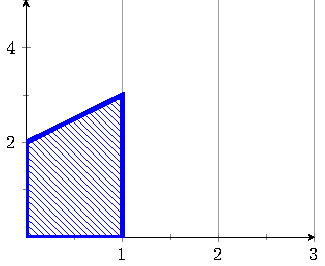
\includegraphics[width=0.4\linewidth]{hinh2.pdf}
        \caption{Tập nghiệm của bài toán $(P_1)$}
    \end{figure}
\end{frame}

\begin{frame}
    \begin{itemize}
    \item <1-> Tương tự bài toán $(P_2)$ ta được $x^{(2)}_1 = 2, x^{(2)}_2 = 0.5$ và $z_2=12.05$.
    \bigskip
    \item <2-> Chọn $x^{(2)}_2 = 0.5$ để cải thiện phương án. Ta được 2 bài toán con $(P_3)$ và $(P_4)$:
    \end{itemize}
    \bigskip
    \begin{columns}
\begin{column}{0.5\textwidth}<2->
    \small
    \begin{equation*}
        \begin{split}
            (P_3) \quad &z_3= 5.5x^{(3)}_1 + 2.1x^{(3)}_2 \\
            & \left\{\begin{array} {cccc}
             -x^{(3)}_1 &+ x^{(3)}_2 &\leq& 2 \\
             8x^{(3)}_1 &+ 2x^{(3)}_2 &\leq& 17 \\
             \color{blue} x^{(3)}_1&& \color{blue}\geq &\color{blue}2 \\
             &\color{blue} x^{(3)}_2& \color{blue}\leq& \color{blue}0 \\
            x^{(3)}_1 &&\geq &0 \\
            &x^{(3)}_2 &\geq &0. \\
            \end{array}\right. \\
        \end{split}
    \end{equation*}
\end{column}
\begin{column}{0.5\textwidth}<2->
   \small
   \begin{equation*}
        \begin{split}
            (P_4) \quad &z_4= 5.5x^{(4)}_1 + 2.1x^{(4)}_2  \\
            & \left\{\begin{array} {cccc}
             -x^{(4)}_1 &+ x^{(4)}_2 &\leq& 2 \\
             8x^{(4)}_1 &+ 2x^{(4)}_2 &\leq& 17 \\
             \color{blue} x^{(4)}_1 &&\color{blue}\geq& \color{blue}2 \\
             &\color{blue} x^{(4)}_2 &\color{blue}\geq&\color{blue} 1 \\
            x^{(4)}_1 &&\geq& 0 \\
            &x^{(4)}_2 &\geq& 0. \\
            \end{array}\right. \\
        \end{split}
    \end{equation*}
\end{column}
\end{columns}
\end{frame}

\begin{frame}
    \begin{itemize} 
    \item<1-> Giải bài toán $(P_3)$ ta được $x^{(3)}_1=2.125, x^{(3)}_2=0$ và $z_3=11.6875 \Rightarrow $ không khả thi do $z_3 < z_1$ \textbf{(gọt bởi cận)}. 
    \medskip
    \item<1-> Bài toán $(P_4)$ \textbf{vô nghiệm}.
    \bigskip
    \item<2-> Vậy phương án tối ưu của bài toán là $x^{(1)}_1=1, x^{(1)}_2=3$ và $z=11.8$.
\end{itemize}
\end{frame}

\begin{frame}{Sơ đồ thuật toán}
\begin{itemize}
\item<1-> Ta gọi bài toán $(P)$ có nút ban đầu là $N_0$, tương ứng mỗi bài toán tối ưu tuyến tính thông thường $(P_i)$ ứng với mỗi nút $N_i$ trên sơ đồ nhánh và $\mathcal{L}$ là danh sách chứa các nút được lập thông qua lý thuyết xác định cận và lý thuyết nghiệm.
\bigskip
\item<2-> Ta đánh dấu giá trị tối ưu tốt nhất và nghiệm tối ưu tốt nhất của bài toán lần lượt là $z^*$ và $(x^*,y^*)$.
\end{itemize}
\end{frame}

\begin{frame}{Sơ đồ thuật toán}
\small
\setlength{\parindent}{4em}
\onslide<1->{\noindent \textbf{Bước 1. Thiết lập} \\
Đặt $\mathcal{L}:=\{N_0 \}$, $z^*=z_p$ và $(x^*,y^*)=(x,y)$. \\}
\onslide<2->{\noindent \textbf{Bước 2. Kiểm tra} \\
Nếu $\mathcal{L} = \emptyset$ thì nghiệm tối ưu của bài toán là $(x^*,y^*)$, giá trị \\ tối ưu là $z^*$ và bài toán được giải. \\
Nếu $\mathcal{L} \neq \emptyset$, chuyển sang bước 3. \\}
\onslide<3->{\noindent \textbf{Bước 3. Chọn nút} \\
Chọn nút $N_i$ từ danh sách $\mathcal{L}$ và xoá khỏi $\mathcal{L}$ sau đó chuyển sang \\ bước 4. \\}
\onslide<4->{\noindent \textbf{Bước 4. Xác định cận} \\ 
Giải bài toán $(P_i)$, nếu bài toán vô nghiệm hoặc $z_i \leq z^*$, quay \\ lại bước 2, nếu không, chuyển sang bước 5. \\}
\onslide<5->{\noindent \textbf{Bước 5. Gọt nghiệm} \\
Nếu tồn tại $x^{(i)} \notin Z^n_+$, ta thêm nút $N_{i+1}, \ldots , N_{k}$ vào $\mathcal{L}$ và quay \\ về bước 2. \\
Nếu không tồn tại $x^{(i)} \notin Z^n_+$, tức $\forall x^{(i)} \in Z^n_+$, ta đặt $z_i = z^*$, \\ $(x^{(i)},y^{(i)}) = (x^*,y^*)$ và quay lại bước 2.}
\end{frame}    

\begin{frame}{Sơ đồ thuật toán}
\center
\begin{figure}
\begin{tikzpicture}[scale=0.33, every node/.style={scale=0.33}, node distance=4cm]
% Define styles
\tikzstyle{startstop} = [rectangle, rounded corners, minimum width=1cm, minimum height=1cm, align=center, draw=black, fill=red!30]
\tikzstyle{process} = [rectangle, minimum width=1cm, minimum height=1cm, align=center, draw=black, fill=orange!30]
\tikzstyle{decision} = [diamond, aspect=2, minimum width=1cm, minimum height=1cm, align=center, draw=black, fill=green!30]
\tikzstyle{io} = [trapezium, trapezium left angle=70, trapezium right angle=110, minimum width=1cm, minimum height=1cm, align=center, draw=black, fill=blue!30]
\tikzstyle{arrow} = [thick,->,>=stealth,line width=0.2pt]
% Place nodes
\node (start) [startstop, xshift=-5cm] {Bắt đầu};
\node (b0) [io, right of=start] {$\mathcal{L}:=\{N_0 \}$ \\ $z^*=z_p$ \\ $(x^*,y^*)=(x,y)$};
\node (b1) [decision, right of=b0] {$\mathcal{L} = \emptyset$?};
\node (b2) [process, right of=b1] {Chọn $N_i$ từ $\mathcal{L}$ \\ và xoá khỏi $\mathcal{L}$};
\node (b3) [process, right of=b2] {Giải $(P_i)$};
\node (b4) [decision, right of=b3] {Vô nghiệm?};
\node (b5) [decision, right of=b4] {$\exists x^{(i)} \notin Z^n_+$?};
\node (b6) [io, above of=b5] {$z_i = z^*$, $(x^{(i)},y^{(i)}) = (x,y)$};
\node (b7) [io, right of=b5] {Thêm \\ $N_{i1}, \ldots , N_{ik}$ \\ vào $\mathcal{L}$};
\node (stop) [startstop, right of=b7] {Kết thúc};
% Draw arrows
\draw [arrow] (start) -- (b0);
\draw [arrow] (b0) -- (b1);
\draw [arrow] (b1) -- node[anchor=south] {no} (b2);
\draw [arrow] (b2) -- (b3);
\draw [arrow] (b3) -- (b4);
\draw [arrow] (b4) -- node[anchor=south] {no} (b5);
\draw [arrow] (b5) -- node[anchor=west] {no} (b6);
\draw [arrow] (b5) -- node[anchor=south] {yes} (b7);
\draw [arrow] (b4) --node[anchor=west] {yes} (15,2) -- (3,2) -- (b1);
\draw [arrow] (b6) -| (b1);
\draw [arrow] (b7) -- (23,6) -- (3,6) -- (b1);
\draw [arrow] (b7) -- (stop);
\draw [arrow] (b1) -- node[anchor=west] {yes} (3,-3) -| (stop);
\end{tikzpicture}
\caption{Lưu đồ giải thuật của thuật toán nhánh cận.}
\end{figure}
\end{frame}   





\section{Kết luận và Hướng phát triển}
\begin{frame}{Tóm tắt kết quả thu được}
\onslide<1->{Đề tài nghiên cứu này đạt được các vấn đề sau đây:}
\bigskip
\begin{itemize}
    \item<2-> Giới thiệu một cách rõ ràng về bài toán \textbf{tối ưu tuyến tính cho ra nghiệm nguyên}.
    \medskip
    \item<3-> Trình bày về ý tưởng \textbf{lát cắt và thuật toán Gomory} để giải bài toán tối ưu nguyên.
    \medskip
	\item<4-> Tìm hiểu về \textbf{phương pháp Land-Doig} hay còn gọi là \textbf{phương pháp nhánh cận}, một phương pháp giúp giải bài toán tối ưu tuyến tính nguyên khả thi trên máy tính và mang tính ứng dụng cao.
\end{itemize}
\end{frame}
\section*{Vấn đề và thách thức}
\begin{frame}{Hạn chế của phương pháp Land-Doig}
\begin{itemize}
    \item<1-> \textbf{Thời gian tính toán lớn}: Việc phân nhánh tạo ra nhiều bài toán con, dẫn đến tăng chi phí tính toán.
    \item<2-> \textbf{Bộ nhớ tiêu tốn lớn}: Quá trình phân nhánh và lưu trữ các nhánh mở rộng tiêu tốn nhiều bộ nhớ, đặc biệt là với những bài toán có kích thước lớn.
    \item<3-> \textbf{Phụ thuộc vào chiến lược phân nhánh}: Hiệu quả của thuật toán phụ thuộc vào cách chọn nhánh để phân chia (cách chọn biến, cận).
    \item<4-> \textbf{Khó khăn trong đánh giá ràng buộc cận}: Việc đánh giá cận không luôn chính xác, dẫn đến khó xác định nhánh nào cần loại bỏ sớm.
    \item<5-> \textbf{Hiệu quả giảm dần với bài toán có nhiều ràng buộc}: Số lượng nhánh cần mở rộng có xu hướng tăng mạnh khi có nhiều ràng buộc, gây giảm hiệu quả.
\end{itemize}
\end{frame}

\section*{Hướng phát triển trong tương lai}
\section*{Học Máy (Machine learning)}

\begin{frame}{Tối ưu hóa Thuật toán Land-Doig bằng phương pháp Học Máy}
    \onslide<1->{Trong quá trình giải quyết bài toán tối ưu tuyến tính nguyên, đặc biệt với các bài toán có \textcolor{red}{\textbf{kích thước lớn}}, việc quyết định lựa chọn phân nhánh nào cho một nút nhất định vẫn là một vấn đề nan giải và chưa có giải pháp hiệu quả.}
    
    \bigskip

    \onslide<2->{\textbf{Phương pháp Học máy (Machine learning)} giúp mang đến một hướng tiếp cận tiềm năng bằng cách cải thiện quy trình chọn nhánh bằng cách sử dụng dữ liệu để xác định các nhánh triển vọng, qua đó tăng tốc quá trình giải các bài toán tối ưu tuyến tính nguyên.\footfullcite{Deza_2023}}
\end{frame}

\section*{Tối ưu phân thức tuyến tính cho nghiệm nguyên}

\begin{frame}{Tối ưu phân tuyến tính (Linear-Fractional Programming)}
    \begin{equation} \small \label{F}
        \begin{split}
        \onslide<1->{(F) \quad Q(x) & = \frac{P(x)}{D(x)} \quad \longrightarrow Max \\
            & \left\{
            \begin{split}
            &Ax \leq  b, \\
            &x \geq 0. \\
            \end{split}
            \right.}
        \end{split}
    \end{equation}            
    \begin{itemize} \small
    \item<2-> Bài toán $(F)$ gọi là bài toán \textbf{Tối ưu phân tuyến tính.}
    \item<3-> Trong đó $A$ là ma trận $m\times n$, $b=\begin{pmatrix}
        b_1 \\
        b_2 \\
        \vdots \\
        b_m
        \end{pmatrix}$, với $x\in \mathbb{R}^n_+$. Tập $S_F:=\{x\in \mathbb{R}^n_+: Ax\leq b\}$ là tập nghiệm của bài toán Tối ưu phân tuyến tính. 
    \item<4-> $P(x)=p^Tx+p_0$, với $p^T = (p_1 \: p_2 \: \ldots \: p_n)$ và $D(x)=d^Tx+d_0$, với $d^T = (d_1 \: d_2 \: \ldots \: d_n)$ ($D(x)>0, \forall x \in S_F$).
    \end{itemize}
\end{frame}







\begin{frame}{Tối ưu phân tuyến tính nguyên hoàn toàn}
\begin{equation} \small
    \begin{split}
    (H) \quad Q(x) & = \frac{P(x)}{D(x)} \quad \longrightarrow Max \\
        & \left\{
        \begin{split}
        &Ax \leq  b, \\
        &x \geq 0, \text{nguyên} \\
        \end{split}
        \right.    
    \end{split}
\end{equation}            
\begin{itemize} \small
\item Bài toán $(H)$ gọi là bài toán \textbf{Tối ưu phân tuyến tính nguyên hoàn toàn.}
\item Trong đó $A$ là ma trận $m\times n$, $b=\begin{pmatrix}
    b_1 \\
    b_2 \\
    \vdots \\
    b_m
    \end{pmatrix}$, với $x\in \mathbb{Z}^n_+$. Tập $S_h:=\{x\in \mathbb{Z}^n_+: Ax\leq b\}$ là tập nghiệm của bài toán Tối ưu phân tuyến tính nguyên hoàn toàn. 
\item $P(x)=p^Tx+p_0$, với $p^T = (p_1 \: p_2 \: \ldots \: p_n)$ và $D(x)=d^Tx+d_0$, với $d^T = (d_1 \: d_2 \: \ldots \: d_n)$ ($D(x)>0, \forall x \in S_h$).
\end{itemize}
\end{frame}
\begin{frame}
    \begin{figure}[h]
        \centering
        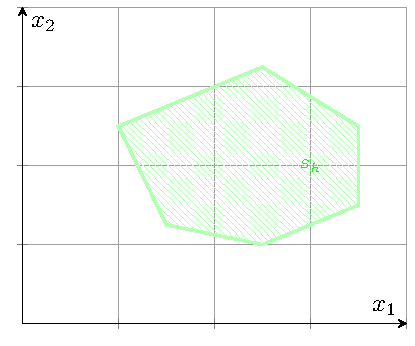
\includegraphics[width=0.65\linewidth]{iflphoantoan.pdf}
        \caption{Tập nghiệm minh hoạ của bài toán (H)}
    \end{figure}
\end{frame}


\begin{frame}{Tối ưu phân tuyến tính nguyên bộ phận}
\vspace{-1cm}
\large
\begin{equation}
    \begin{split}
    (B) \quad Q(x,y) & = \frac{P(x,y)}{D(x,y)} \quad \longrightarrow Max \\
        & \left\{
        \begin{split}
        &Ax + Gy \leq  b, \\
        &x \geq 0, \text{nguyên} \\
        &y \geq 0.
        \end{split}
        \right.    
    \end{split}
\end{equation}            
\end{frame}
\begin{frame}
\begin{itemize}
\item Bài toán $(B)$ gọi là bài toán \textbf{Tối ưu phân tuyến tính nguyên bộ phận.}
\medskip
\item Trong đó $A$ là ma trận $m\times n$, $G$ là ma trận $m\times t$, $b=\begin{pmatrix}
    b_1 \\
    b_2 \\
    \vdots \\
    b_m
    \end{pmatrix}$, với $x\in \mathbb{Z}^n_+$ và $y \in \mathbb{R}^t_+$. Tập $S_b:=\{(x,y)\in \mathbb{Z}^n_+ \times \mathbb{R}^t_+: Ax+Gy\leq b\}$ là tập nghiệm của bài toán Tối ưu phân tuyến tính nguyên bộ phận. 
\medskip
\item $P(x,y)=p^T_1x+p^T_2y+p_0$, với $p^T_1 = (p_1 \: p_2 \: \ldots \: p_n)$ và $p^T_2 = (p_1 \: p_2 \: \ldots \: p_t)$.
\medskip
\item $D(x,y)=d^T_1x+d^T_2y+d_0$, với $d^T_1 = (d_1 \: d_2 \: \ldots \: d_n)$ và $d^T_2 = (d_1 \: d_2 \: \ldots \: d_t)$ ($D(x,y)>0, \forall x \in S_b$).
\end{itemize}
\end{frame}
\begin{frame}
    \onslide<1->{\begin{figure}[h]
        \centering
        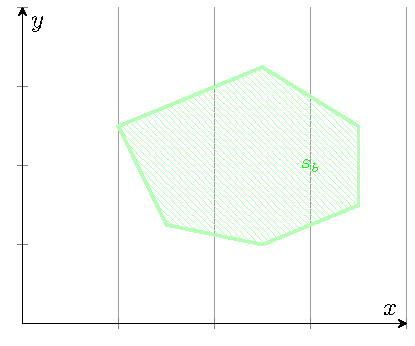
\includegraphics[width=0.4\linewidth]{iflpbophan.pdf}
        \caption{Tập nghiệm minh hoạ của bài toán (B)}
    \end{figure}}

    \bigskip
    \onslide<2->{Có một lý thuyết riêng cho việc xử lý các bài toán Tối ưu phân thức tuyến tính và \textcolor{red}{tìm nghiệm nguyên.}\footfullcite{bajalinov2013linear}}
\end{frame}





\begin{frame}[allowframebreaks, noframenumbering]
    \nocite{*}
    \printbibliography
\end{frame}


\begin{frame}
    \begin{block}{}
    \medskip
    \center{\huge \it \textcolor[rgb]{0.50,0.30,1.0}{Cảm ơn quý thầy cô và các anh chị đã quan tâm theo dõi!}}
    \medskip
    \end{block}	
\end{frame}    
\end{document}
